%\documentclass[presentation]{beamer}
\documentclass[aspectratio=169]{beamer}
\usepackage{amsmath,amsthm, amssymb, latexsym}
\usepackage{amssymb}
\usepackage{graphicx}
\usepackage[absolute,overlay]{textpos}

\usepackage{dirtytalk}

\usepackage{booktabs}

\usepackage{colortbl}



\usepackage{tikz}
\usetikzlibrary{arrows.meta,calc}
\usepackage{neuralnetwork}

\usepackage[most]{tcolorbox}

\usetikzlibrary{matrix}

\usetikzlibrary{arrows}


\usepackage{graphicx}

\usepackage{mathtools}
\usepackage{bm}

\usepackage{dsfont}




\usepackage{times}
\usepackage{tikz}
\usepackage{amsmath}
\usepackage{verbatim}
\usetikzlibrary{arrows,shapes}
\usepackage{varwidth}
\usepackage{pgfplots}
\usetikzlibrary{%
	arrows,%
	automata,%
	calc,%
	patterns,%
	plotmarks,%
	positioning,%
	shapes.geometric,%
	shapes,%
	snakes,%
}

\usepackage{graphicx} % Allows including images
\usepackage{booktabs} % Allows the use of \toprule, \midrule and \bottomrule in tables

\tikzstyle{na} = [baseline=-.5ex]


\DeclareMathOperator{\tr}{tr}

%COLORS
\definecolor{bleudefrance}{rgb}{0.19, 0.55, 0.91}

\definecolor{davysgrey}{rgb}{0.33, 0.33, 0.33}

%%End Rawad


\setbeamertemplate{footline}{%
    \raisebox{5pt}{\makebox[\paperwidth]{\hfill\makebox[25pt]{\color{gray}
          \scriptsize\insertframenumber }}}\hspace*{5pt}}





\newcommand{\bigCI}{\mathrel{\text{\scalebox{1.07}{$\perp\mkern-10mu\perp$}}}}
\newcommand{\argmax}{\operatornamewithlimits{argmax}} 
\newcommand{\Inf}{\operatorname{Inf}}
\newcommand{\Var}{\operatorname{Var}}  
\newcommand{\Maj}{\operatorname{Maj}} 
\newcommand{\dist}{\operatorname{dist}} 

\setbeamertemplate{navigation symbols}{}

\setbeamercolor{block title}{use=structure,fg=white,bg=blue!75!black}
\setbeamercolor{block body}{use=structure,fg=black,bg=blue!20!white}

\setbeamercolor{block title example}{use=structure,fg=white,bg=green!40!black}
\setbeamercolor{block body example}{use=structure,fg=black,bg=green!10!white}



\newcommand\FourQuad[4]{%
 \begin{minipage}[b][.33\textheight][t] 
  {.48\textwidth}#1\end{minipage}\hfill%
 \begin{minipage}[b][.33\textheight][t] 
  {.48\textwidth}#2\end{minipage}\\[0.5em]
 \begin{minipage}[b][.33\textheight][t] 
  {.48\textwidth}#3\end{minipage}\hfill
 \begin{minipage}[b][.33\textheight][t] 
  {.48\textwidth}#4\end{minipage}%
 }
 





\DeclareMathOperator{\terms}{terms}

\newcommand{\interior}[1]{%
  {\kern0pt#1}^{\mathrm{o}}%
}

% \setbeamertemplate{itemize item}{\color{blue!75!black}$\bullet$}
% \setbeamertemplate{itemize subitem}{\color{blue!75!black}$\circ$}


\title{\textbf{\textit{HerA} Scheme: Secure Distributed Matrix Multiplication via Hermitian Codes}}
\author[]{Roberto Assis Machado$^1$\\
Welington Santos$^2$\\
Gretchen L. Matthews$^2$}
\institute{$^1$ Clemson University\\
$^2$ Virginia Tech}
\date{January 7, 2023}


\begin{document}

\begin{frame}
\titlepage


\end{frame}


\begin{frame}{Secure Distributed Matrix Multiplication (SDMM)}

\begin{columns}
\begin{column}{0.5\textwidth}
        \resizebox{7.5cm}{!}{
\begin{tikzpicture}
\definecolor{darkturquoise}{rgb}{0.0, 0.81, 0.82}
\node[rectangle, rounded corners = 3mm, draw = black, minimum height = 0.6cm, fill =white] (m) at (0,0) {\small User}; 


\node[rectangle,  draw = black!60, fill = bleudefrance, minimum height = 1.2 cm, minimum width = 0.5cm, opacity=.5, text opacity=1 ,above right = -0.2 and 0.5 cm of m] (a) {\small $A$};

\node[rectangle,  draw = black!60, fill = green!50!black, minimum height = 0.5 cm, minimum width = 1.2 cm, opacity=.5, text opacity=1 , right = 0.1 cm of a.north east, anchor = north west] (b) {\small $B$};



%\node[rectangle,  draw = black!60, fill = bleudefrance, minimum height = 1.1 cm, minimum width = 0.45cm, opacity=.5, text opacity=1, left = 0 cm of eq] (a) {\small $X$};%of a1.north west, anchor = north east] (a) 

\node[rectangle, rounded corners = 1mm, draw = black, minimum height = 0.6 cm, minimum width = 1 cm,  fill = white, below = 1.8 cm of m.south west, anchor = north east] (w2) {\scriptsize Server $2$};
\node[rectangle, rounded corners = 1mm, draw = black, minimum height = 0.6 cm, minimum width = 1 cm, fill = white, left = 0.8 cm of w2] (w1) {\scriptsize Server $1$};
\node[right = 0.1 cm of w2] (d) {$\cdots$};
\node[rectangle, rounded corners = 1mm, draw = black, minimum height = 0.6 cm, minimum width = 1 cm, fill = white, right = 1 cm of w2] (w4) {\scriptsize Server $N-1$};
\node[right = 0.1 cm of w2] (d) {$\cdots$};
\node[rectangle, rounded corners = 1mm, draw = black, minimum height = 0.6 cm, minimum width = 1 cm, fill = white, right = 0.8 cm of w4] (w3) {\scriptsize Server $N$};

\node[rectangle,  draw = black!60, fill = bleudefrance, minimum height = 0.3 cm, minimum width = 0.5 cm, opacity=.5, text opacity=1, below right = 0.1 and 0.25 cm of w1.south west, anchor = north west] (a11) node[below = 0 of a11, color = bleudefrance] {\begin{varwidth}{0.6cm} \centering \tiny $\Tilde{A}_1$ \end{varwidth}};

\node[rectangle,  draw = black!60, fill = green!50!black, minimum height = 0.5 cm, minimum width = 0.3 cm, opacity=.5, text opacity=1, right = 0.1 cm of a11.north east, anchor = north west] (b11) node[below = 0 of b11, color = green!50!black] {\begin{varwidth}{0.6cm} \centering \tiny $\Tilde{B}_1$ \end{varwidth}};

\node[rectangle,  draw = black!60, fill = bleudefrance, minimum height = 0.3 cm, minimum width = 0.5 cm, opacity=.5, text opacity=1, below right = 0.1 and 0.25 cm of w2.south west, anchor = north west] (a12) node[below = 0 of a12, color = bleudefrance] {\begin{varwidth}{0.6cm} \centering \tiny $\Tilde{A}_2$ \end{varwidth}};

\node[rectangle,  draw = black!60, fill = green!50!black, minimum height = 0.5 cm, minimum width = 0.3 cm, opacity=.5, text opacity=1, right = 0.1 cm of a12.north east, anchor = north west] (b12) node[below = 0 of b12, color = green!50!black] {\begin{varwidth}{0.6cm} \centering \tiny $\Tilde{B}_2$ \end{varwidth}};

\node[rectangle,  draw = black!60, fill = bleudefrance, minimum height = 0.3 cm, minimum width = 0.5 cm, opacity=.5, text opacity=1, below right = 0.1 and 0.5 cm of w4.south west, anchor = north west] (a14) node[below = 0 of a14, color = bleudefrance] { \tiny $\Tilde{A}_{N-1}$};

\node[rectangle,  draw = black!60, fill = green!50!black, minimum height = 0.5 cm, minimum width = 0.3 cm, opacity=.5, text opacity=1, right = 0.1 cm of a14.north east, anchor = north west] (b14) node[below = 0 of b14.south west, anchor = north west, color = green!50!black] { \tiny $\Tilde{B}_{N-1}$};

\node[rectangle,  draw = black!60, fill = bleudefrance, minimum height = 0.3 cm, minimum width = 0.5 cm, opacity=.5, text opacity=1, below right = 0.1 and 0.25 cm of w3.south west, anchor = north west] (a13) node[below = 0 of a13, color = bleudefrance] {\begin{varwidth}{0.6cm} \centering \tiny $\Tilde{A}_N$ \end{varwidth}};

\node[rectangle,  draw = black!60, fill = green!50!black, minimum height = 0.5 cm, minimum width = 0.3 cm, opacity=.5, text opacity=1, right = 0.1 cm of a13.north east, anchor = north west] (b13) node[below = 0 of b13, color = green!50!black] {\begin{varwidth}{0.6cm} \centering \tiny $\Tilde{B}_N$ \end{varwidth}};

\path
(w1.north) edge (m)
(w2) edge  (m)
(w4) edge (m)
(w3.north) edge  (m);


\end{tikzpicture}
}
\end{column}
\begin{column}{0.5\textwidth}  %%<--- here
    \begin{itemize}
        \item User has two matrices $A$ and $B$ and wants their product $AB$.
        \medskip
        \item $N$ helper servers. 
        \medskip
        \item Want information-theoretic privacy even if $T$ servers collude.
        \medskip
        \item \textbf{Goal:} Speed up computational time.
    \end{itemize}
\end{column}
\end{columns}

\begin{textblock}{20}(0.4,15)
{\tiny \color{davysgrey} W. Chang and R. Tandon, \say{On the Capacity of Secure Distributed Matrix Multiplication,} IEEE GLOBECOM, 2018.}
\end{textblock}

\end{frame}


\begin{frame}{(Some of the) Previous Literature}

\begin{itemize}
    
    \item {\scriptsize \color{davysgrey} J. Kakar, S. Ebadifar, and A. Sezgin \say{On the capacity and straggler robustness of distributed secure matrix multiplication,} IEEE Access, 2019.}
   
    \item {\scriptsize \color{davysgrey} H. Esfahanizadeh, A. Cohen, M. Médard, and S. Shamai, \say{Distributed Computations with Layered Resolution,} in arXiv 2208.01437v1, 2022.}
        
    \item {\scriptsize \color{davysgrey} Q. Yu, S. A. Avestimehr, \say{Entangled polynomial codes for secure, private, and batch distributed matrix multiplication: Breaking the cubic barrier,} IEEE ISIT, 2020.}
        
    \item {\scriptsize \color{davysgrey} N. Mital, L. Cong, and G. Deniz, \say{Secure Distributed Matrix Computation With Discrete Fourier Transform,} IEEE Transactions on Information Theory, 2022.}
    
    \item {\scriptsize \color{davysgrey} H. López; G. Matthews; D. Valvo, \say{Secure MatDot codes: a secure, distributed matrix multiplication scheme,} IEEE ITW, 2022.}
        
    \item {\scriptsize \color{davysgrey} R. G. L. D'Oliveira, S. El Rouayheb, D. Heinlein and D. Karpuk, \say{Degree Tables for Secure Distributed Matrix Multiplication,} IEEE JSAIT, 2021.}
        
        
   % \item {\scriptsize \color{davysgrey} S. Kadhe and A. Sprintson, \say{Weakly secure regenerating codes for distributed storage,}2014 International Symposium on Network Coding (NetCod), 2014.}
        
\end{itemize}


    
\end{frame}



\begin{frame}{Focus on Minimizing Number of Servers and Communication Costs}

\begin{itemize}
    \item Previous work focused on reducing the number of servers as a proxy for minimizing communication costs.
    
    \medskip
    
    \item<2-> Adapted technique from repairing Reed-Solomon codes allowed to reduce the total communication while increasing  the number of servers. 
    
    \medskip
    
    \item<3-> Most of those techniques requires to perform in ``large'' finite fields.
    
    \medskip
    
    \item<3-> Hermitian Codes are employed to significantly reduce the size of the finite fields without compromising security and computational complexity.
    
\end{itemize}

% \uncover<4->{
% \begin{textblock}{20}(0.4,14.4)
% {\tiny \color{davysgrey} *V. Guruswami and M. Wootters, \say{Repairing Reed-Solomon codes,} IEEE Transactions on Information Theory, 2017.}
% \end{textblock}
% \begin{textblock}{20}(0.4,15)
% {\tiny \color{davysgrey} *I. Tamo, M. Ye, and A. Barg, \say{Optimal repair of reed-solomon codes:
% Achieving the cut-set bound,} IEEE FOCS, 2017.}
% \end{textblock}
% }

    
\end{frame}


\begin{frame}{Discrete Fourier Transform (DFT) Code for $N=4$ Servers}

\begin{figure}
\centering

\resizebox{!}{4cm}{
\begin{tikzpicture}
\definecolor{darkturquoise}{rgb}{0.0, 0.81, 0.82}

\node[rectangle, rounded corners = 3mm, draw = black, minimum height = 0.6cm, fill =white] (m) at (0,0) {{User}}; 

\node[rectangle,  draw = black!60, fill = bleudefrance, minimum height = 1.2 cm, minimum width = 0.5cm, opacity=.5, text opacity=1 ,above right = -0.2 and 0.5 cm of m] (a) { \small \begin{bmatrix}
A_1 & A_2
\end{bmatrix}};

\node[rectangle,  draw = black!60, fill = green!50!black, minimum height = 0.5 cm, minimum width = 1.2 cm, opacity=.5, text opacity=1 , right = 0.1 cm of a.north east, anchor = north west] (b) {\small \begin{bmatrix}
B_1 \\  B_2
\end{bmatrix}};


\node[rectangle, rounded corners = 1mm, draw = black, minimum height = 0.6 cm, minimum width = 1 cm,  fill = white] (w2) at (-1.3,-3) {Server $2$};

\node[rectangle, rounded corners = 1mm, draw = black, minimum height = 0.6 cm, minimum width = 1 cm, fill = white, left = 1 cm of w2] (w1) {Server $1$};

\node[rectangle, rounded corners = 1mm, draw = black, minimum height = 0.6 cm, minimum width = 1 cm, fill = white, right = 1 cm of w2] (w3) {Server $3$};

\node[rectangle, rounded corners = 1mm, draw = black, minimum height = 0.6 cm, minimum width = 1 cm, fill = white, right = 1 cm of w3] (w4) {Server $4$};

% \node[minimum height = 0.45 cm, minimum width = 2cm, opacity=.5, text opacity=1, below = 0.1cm of w1] (a11) { \centering \small \uncover<4->{$h(1)=f(1)g(1)$} };

% \node[minimum height = 0.45 cm, minimum width = 0.6cm, opacity=.5, text opacity=1, below = 0.1cm of w2] (a22) { \centering \small \uncover<4->{$h(2)=f(2)g(2)$} };

% \node[minimum height = 0.45 cm, minimum width = 0.6cm, opacity=.5, text opacity=1, below = 0.1cm of w3] (a33) { \centering \small \uncover<4->{$h(3)=f(3)g(3)$} };
\uncover<2->{
\node[rectangle,  draw = black!60, fill = bleudefrance, minimum height = 0.3 cm, minimum width = 0.5 cm, opacity=.5, text opacity=1, below right = 0.1 and 0.25 cm of w1.south west, anchor = north west] (a11);

\node[rectangle,  draw = black!60, fill = bleudefrance, minimum height = 0.3 cm, minimum width = 0.5 cm, opacity=.5, text opacity=1, below right = 0.1 and 0.25 cm of w4.south west, anchor = north west] (a14);

%\node[rectangle,  draw = black!60, fill = green!50!black, minimum height = 0.5 cm, minimum width = 0.3 cm, opacity=.5, text opacity=1, right = 0.1 cm of a14.north east, anchor = north west] (b11) node[below = 0 of b11, color = green!50!black] (c11) {\begin{varwidth}{0.6cm} \centering \small $g(1)$ \end{varwidth}} %

\node[rectangle,  draw = black!60, fill = green!50!black, minimum height = 0.5 cm, minimum width = 0.3 cm, opacity=.5, text opacity=1, right = 0.1 cm of a11.north east, anchor = north west] (b11) node[below = 0 of b11, color = green!50!black] (c11) {\begin{varwidth}{0.6cm} \centering \small $g(\alpha_1)$ \end{varwidth}} %
node[left = -0.2 of c11.west, anchor = east, color = bleudefrance] { \centering \small %\uncover<4->{ {\color{magenta}$h(0)=$}}
{\color{bleudefrance}$f(\alpha_1)$}};
%node[left = 0.3 of c11.west, anchor = east, color = magenta] { \small ;

\node[rectangle,  draw = black!60, fill = bleudefrance, minimum height = 0.3 cm, minimum width = 0.5 cm, opacity=.5, text opacity=1, below right = 0.1 and 0.25 cm of w2.south west, anchor = north west] (a12);


\node[rectangle,  draw = black!60, fill = green!50!black, minimum height = 0.5 cm, minimum width = 0.3 cm, opacity=.5, text opacity=1, right = 0.1 cm of a12.north east, anchor = north west] (b12) node[below = 0 of b12, color = green!50!black] (c12) {\begin{varwidth}{0.6cm} \centering \small $g(\alpha_2)$ \end{varwidth}} %
node[left = -0.2 of c12.west, anchor = east, color = bleudefrance] { \centering \small %\uncover<4->{ {\color{magenta}$h(\alpha^5)=$}} 
{\color{bleudefrance}$f(\alpha_2)$}};;


\node[rectangle,  draw = black!60, fill = bleudefrance, minimum height = 0.3 cm, minimum width = 0.5 cm, opacity=.5, text opacity=1, below right = 0.1 and 0.25 cm of w3.south west, anchor = north west] (a13);

\node[rectangle,  draw = black!60, fill = green!50!black, minimum height = 0.5 cm, minimum width = 0.3 cm, opacity=.5, text opacity=1, right = 0.1 cm of a13.north east, anchor = north west] (b13) node[below = 0 of b13, color = green!50!black] (c13) {\begin{varwidth}{0.6cm} \centering \small $g(\alpha_3)$ \end{varwidth}} %
node[left = -0.2 of c13.west, anchor = east, color = bleudefrance] { \centering \small %\uncover<4->{ {\color{magenta}$h(\alpha^{10})=$}} 
{\color{bleudefrance}$f(\alpha_3)$}};;

\node[rectangle,  draw = black!60, fill = bleudefrance, minimum height = 0.3 cm, minimum width = 0.5 cm, opacity=.5, text opacity=1, below right = 0.1 and 0.25 cm of w4.south west, anchor = north west] (a14);
\node[rectangle,  draw = black!60, fill = green!50!black, minimum height = 0.5 cm, minimum width = 0.3 cm, opacity=.5, text opacity=1, right = 0.1 cm of a14.north east, anchor = north west] (b13) node[below = 0 of b13, color = green!50!black] (c13) {\begin{varwidth}{0.6cm} \centering \small $g(\alpha_4)$ \end{varwidth}} %
node[left = -0.2 of c13.west, anchor = east, color = bleudefrance] { \centering \small %\uncover<4->{ {\color{magenta}$h(\alpha^{15})=$}} 
{\color{bleudefrance}$f(\alpha_4)$}};;
}





\path<2-3>[<-]
(w1.north)  edge[bend left] node[above left = 0 cm and -1cm, midway, sloped, font=\small] {$f(\alpha_1),g(\alpha_1)$} (m)
[->]
(m) edge[bend right] node[right = -0.2cm, below=-0.05cm, midway, sloped, font=\small] {$f(\alpha_2),g(\alpha_2)$} (w2)
[<-]
(w3.north) edge[bend right] node[above right = 0 cm and -0.8cm, midway, sloped, font=\small] {$f(\alpha_3),g(\alpha_3)$} (m)
[<-]
(w4.north) edge[bend right] node[above right = 0 cm and -0.8cm, midway, sloped, font=\small] {$f(\alpha_4),g(\alpha_4)$} (m)
;
\path<4->[->, color = magenta]
(w1.north)  edge node[above left = 0 cm and -1cm, midway, sloped, font=\small] {$h(\alpha_1)$} (m)
[<-]
(m) edge node[right = -0.2cm, above=0.05cm, midway, sloped, font=\small] {$h(\alpha_2)$} (w2)
[->]
(w3.north) edge node[above right = 0 cm and -0.8cm, midway, sloped, font=\small] {$h(\alpha_3)$} (m)
[->]
(w4.north) edge node[above right = 0 cm and -0.8cm, midway, sloped, font=\small] {$h(\alpha_4)$} (m)
;
\node<1->[left = 3.5 of m] (v) {$f(x)=A_1+A_2x + Rx^2$};
\node<1->[below = 0 cm of v.south west, anchor = north west] (u)  {$g(x)=B_1+B_2x^{-1}+ S x^{-3}$};
\end{tikzpicture}}


\end{figure}

\begin{itemize}
        \item Generate random  $R$ and $S$ of the same size as $A_i$ and  $B_i$ and form
        $f(x) = A_1 + A_2 x  + Rx^2$ and $g(x) = B_1+B_2x^{-1}+ Sx^{-3}$. 
        \item<2-> User sends $f(\alpha_i)$ and $g(\alpha_i)$ to server $i$.
        \item<3-> $h(x):=f(x)g(x)=A_1B_1+ A_2B_2 + \textit{(non-constants terms)}$
        \item<3-> User wants $AB=A_1B_1+ A_2B_2= h_0$.
        \item<4-> Server $i$ computes $h(\alpha_i)$
        and sends it  to the user.
         \item<5-> User  decodes $AB=\frac{1}{4}\sum_i h(\alpha_i)$, if $4$ divides $q-1$.
    \end{itemize}
\end{frame}



\begin{frame}{Total Communication Rate - DFT Codes}
% \begin{figure}
% \centering
\resizebox{8cm}{!}{
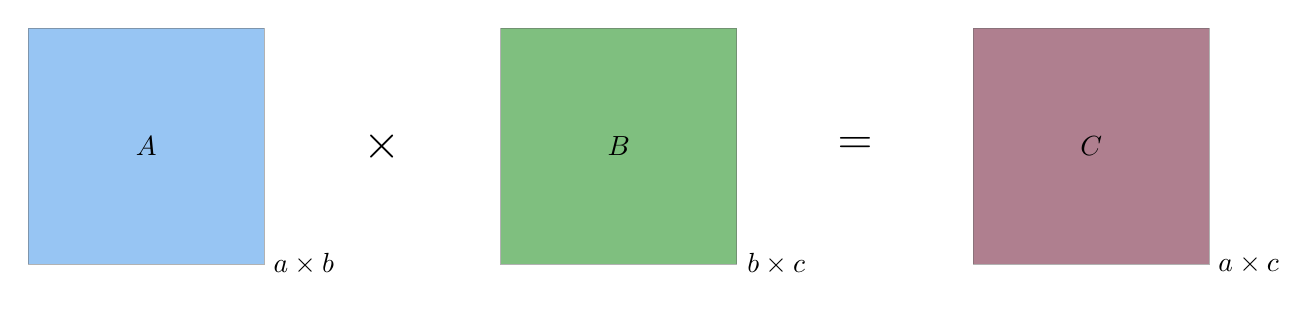
\begin{tikzpicture}
\definecolor{darkturquoise}{rgb}{0.0, 0.81, 0.82}


\node[rectangle,  draw = black!60, fill = bleudefrance, minimum height = 3 cm, minimum width = 3cm, opacity=.5, text opacity=1] (a) at (0,0) { $A$};

\node[] (dim_a) at (2,-1.5) { $a \times b$};

\node[] (times) at (3,0) {\LARGE $\times$};

\node[rectangle,  draw = black!60, fill = green!50!black, minimum height = 3cm, minimum width = 3cm, opacity=.5, text opacity=1] (b) at (6,0) { $B$};

\node[] (dim_b) at (8,-1.5) { $b \times c$};

\node[] (times) at (9,0) {\LARGE $=$};

\node[rectangle,  draw = black!60, fill = purple!50!black, minimum height = 3cm, minimum width = 3cm, opacity=.5, text opacity=1] (c) at (12,0) { $C$};

\node[] (dim_c) at (14,-1.5) { $a \times c$};




\end{tikzpicture}
}
% \end{figure}

\bigskip

\begin{itemize}
    \item<2-> Upload: $2ab + 2bc$ symbols of $\mathbb{F}_{q}$.
    
    \medskip
    
    \item<3-> Download: $4ac$ symbols of $\mathbb{F}_{q}$.
    
    \medskip
    
    \item<4-> Total Communication Rate: $ \mathcal{R} = \dfrac{ac}{2ab+2bc+4ac}$.

    \item<5-> Minimum $q$ is $5$.
\end{itemize}

\bigskip

\bigskip

\uncover<5->{
\textbf{Main Contribution:} Lower the minimum $q$ necessary to perform $AB$ by employing algebraic geometry codes.
}
    
\end{frame}



\begin{frame}{Brief Review - Hermitian Codes}
%\resizebox{9cm}{!}{
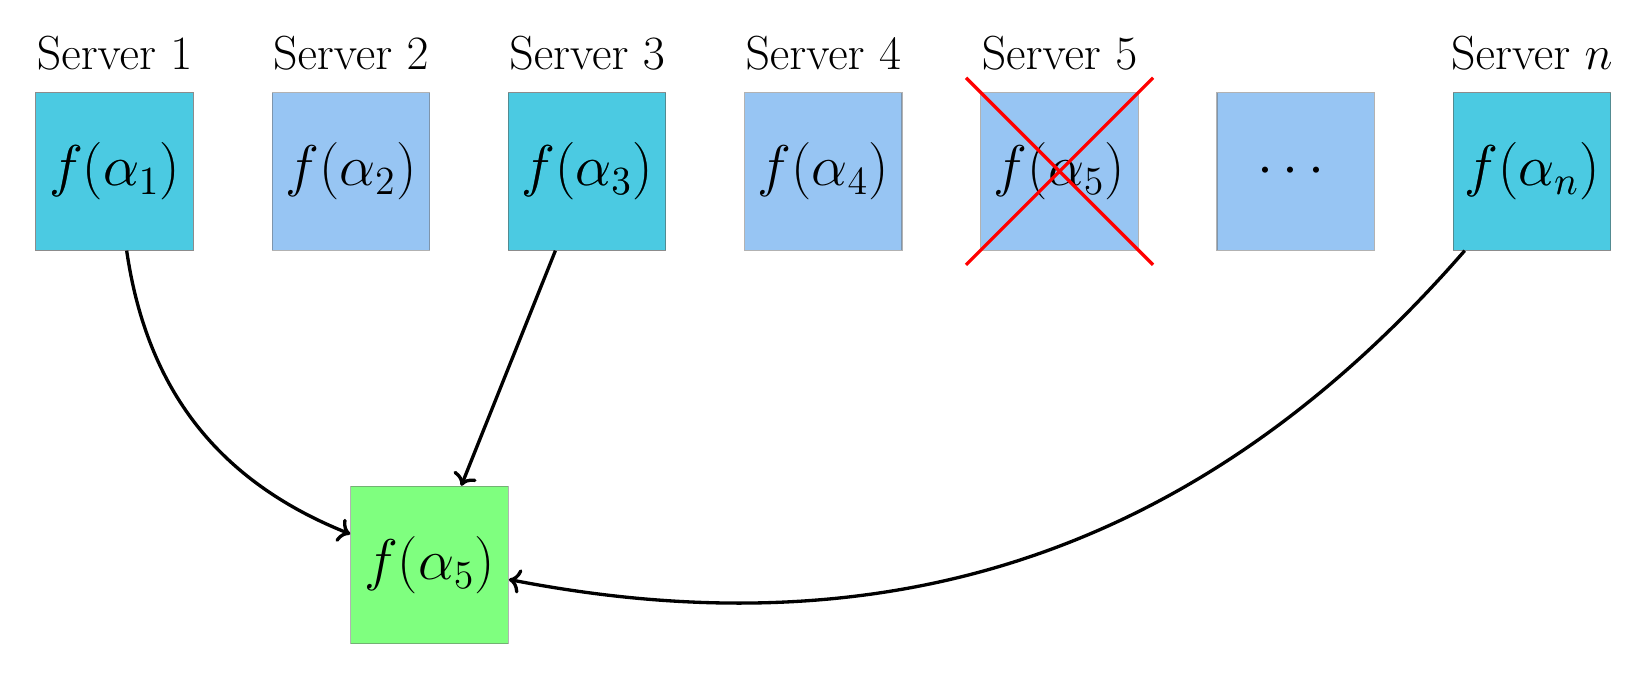
\begin{tikzpicture}
\definecolor{darkturquoise}{rgb}{0.0, 0.81, 0.82}


\tikzset{cross/.style={cross out,very thick, draw=black, minimum size=2*(#1-\pgflinewidth), inner sep=0pt, outer sep=0pt},
%default radius will be 1pt. 
cross/.default={35pt}}


\node[rectangle,  draw = black!60, fill = bleudefrance, minimum height = 2 cm, minimum width = 2cm, opacity=.5, text opacity=1] (a) at (0,0) (F1) { \huge$f(\alpha_1)$};

\node<3->[rectangle,  draw = black!60, fill = darkturquoise, minimum height = 2 cm, minimum width = 2cm, opacity=.5, text opacity=1] (a) at (0,0) (F1) { \huge$f(\alpha_1)$};

\node[] (server1) at (0,1.5) {\LARGE Server $1$};

\node[rectangle,  draw = black!60, fill = bleudefrance, minimum height = 2cm, minimum width = 2cm, opacity=.5, text opacity=1] (b) at (3,0) (F2) {\huge $f(\alpha_2)$};

\node[] (server1) at (3,1.5) {\LARGE Server $2$};

\node[rectangle,  draw = black!60, fill = bleudefrance, minimum height = 2cm, minimum width = 2cm, opacity=.5, text opacity=1] (b) at (6,0) (F3) {\huge $f(\alpha_3)$};

\node<3->[rectangle,  draw = black!60, fill = darkturquoise, minimum height = 2cm, minimum width = 2cm, opacity=.5, text opacity=1] (b) at (6,0) (F3) {\huge $f(\alpha_3)$};

\node[] (server1) at (6,1.5) {\LARGE Server $3$};

\node[rectangle,  draw = black!60, fill = bleudefrance, minimum height = 2cm, minimum width = 2cm, opacity=.5, text opacity=1] (b) at (9,0) {\huge$f(\alpha_4)$ };

\node[] (server1) at (9,1.5) {\LARGE Server $4$};

\node[rectangle,  draw = black!60, fill = bleudefrance, minimum height = 2cm, minimum width = 2cm, opacity=.5, text opacity=1] (b) at (12,0) {\huge$f(\alpha_5)$};

\node[] (server1) at (12,1.5) {\LARGE Server $5$};

\draw<2-> (12,0) node[cross,red] {};


\node[rectangle,  draw = black!60, fill = bleudefrance, minimum height = 2cm, minimum width = 2cm, opacity=.5, text opacity=1] (b) at (15,0) {\huge $\cdots$};



\node[rectangle,  draw = black!60, fill = bleudefrance, minimum height = 2cm, minimum width = 2cm, opacity=.5, text opacity=1] (b) at (18,0) (Fn) {\huge $f(\alpha_n)$};

\node<3->[rectangle,  draw = black!60, fill = darkturquoise, minimum height = 2cm, minimum width = 2cm, opacity=.5, text opacity=1] (b) at (18,0) (Fn) {\huge $f(\alpha_n)$};

\node[] (server1) at (18,1.5) {\LARGE Server $n$};

\uncover<3->{
\node[rectangle,  draw = black!60, fill = green, minimum height = 2cm, minimum width = 2cm, opacity=.5, text opacity=1] (b) at (4,-5) (GF5){\huge$f(\alpha_5)$};
}



\path<3->[->]
(F1)  edge[very thick,bend right] node[above left = 0 cm and -1cm, midway, sloped, font=\small] {} (GF5)
(F3)  edge[very thick] node[above left = 0 cm and -1cm, midway, sloped, font=\small] {} (GF5)
(Fn)  edge[very thick,bend left] node[above left = 0 cm and -1cm, midway, sloped, font=\small] {} (GF5);

\end{tikzpicture}
}
\begin{itemize}
    \item Consider the set of points $\mathcal{P}_{q}(\mathbb{F}_{q^2}):=\left\lbrace P_{\alpha\beta}:\alpha,\beta \in\mathbb{F}_{q^2} : \beta^{q}+\beta=\alpha^{q+1} \right\rbrace$ 
    
    \medskip
    
    \item $\mid \mathcal{P}_{q}(\mathbb{F}_{q^2}) \mid = q^3$
    
    \medskip
    
    \item<2-> Given an integer $m$, consider the subset $\mathcal{L}(mP_{\infty})$ of $\mathbb{F}_{q^2}[x,y]$ generated by $I(m)$, where
    \begin{equation*}
 I(m)=\lbrace x^{i}y^{j}: 0\leq i, 0\leq j\leq q-1, iq+j(q+1)\leq m\rbrace.
\end{equation*}
    \medskip
    
    \item<3-> The $m$-Hermitian Code is \begin{equation*}
\mathcal{C}(mP_{\infty}):=\left\lbrace(f(P_{1}),\ldots,f(P_{n})):f\in\mathcal{L}(mP_{\infty})\right\rbrace.
\end{equation*}
\end{itemize}
%K. Shanmugam, D. S. Papailiopoulos, A. G. Dimakis, and G. Caire, “A repair framework for scalar MDS codes,” IEEE J. Selected Areas Comm. (JSAC), vol. 32, no. 5, pp. 998–1007, 2014.

\end{frame}

\begin{frame}{Fundamental Facts on Hermitian Codes}
%\input{tikz/repair}
\begin{itemize}
    \item For $m\leq q^3+q^2-q-2$. The dual code of the Hermitian code $\mathcal{C}(mP_{\infty})$ is
\begin{equation}
\mathcal{C}(mP_{\infty})^{\perp}=\mathcal{C}(m^{\perp}P_{\infty}),
\end{equation}
with $m^{\perp}=q^3+q^2-q-2-m$.
    \item<2-> $\langle u, v \rangle = 0$, for any $u\in \mathcal{C}(mP_{\infty})$  and $v \in \mathcal{C}(m^{\perp}P_{\infty})$.
\end{itemize}
% \begin{textblock}{21}(0.4,14.4)
% {\tiny \color{davysgrey} V. Guruswami and M. Wootters, \say{Repairing Reed-Solomon codes,} IEEE Transactions on Information Theory, 2017.}
% \end{textblock}
\end{frame}





\begin{frame}{Hermitian Algebraic (HerA) Scheme for $N=4$ Servers}

\begin{figure}
\centering

\input{tikz/hera_example2}


\end{figure}

\begin{itemize}
        \item Generate random  $R$ and $S$ of the same size as $A_i$ and  $B_i$ with entries in $\mathbb{F}_4$ and form
        \begin{equation*}
            \begin{array}{lllll}
f(P_1)=A_{1},&f(P_{2})=A_{2}, &f(P_3)=R&&\\
g(P_1)=B_1, & g(P_2)= B_2, & g(P_3)=S, & g(P_4) = 0, & g(P_5) =0 
\end{array}
        \end{equation*}
    \end{itemize}
\end{frame}


\begin{frame}{Hermitian Algebraic (\textit{HerA}) Scheme for $N=4$ Servers}

\begin{figure}
\centering

\input{tikz/hera_example}


\end{figure}

\begin{itemize}
        \item Generate random  $R$ and $S$ of the same size as $A_i$ and  $B_i$ with entries in $\mathbb{F}_4$ and form
        $f(x, y) = A_1 + (A_1+R+(A_1+A_2)\delta)x+(A_1+A_2)y$ and $g(x,y)= B_1 + (S+B_1\delta^2+B_2)x+(B_1\delta+B_2+S\delta)x^2
+(B_1+B_2)y+(B_1+B_2+S)xy$. 
        \item<2-> User sends $f(P_{i_j})$ and $g(P_{i_j})$ to server $j$.
        \item<3-> $(f(P_1, \ldots, f(P_8))\in \mathcal{C}(3P_\infty)$ and $(g(P_1), \ldots, g(P_8))\in \mathcal{C}(3^\perp P_\infty)= \mathcal{C}(5 P_\infty)$
        \item<3-> User wants $AB=A_1B_1+ A_2B_2= h(P_1) + h(P_2)$.
        \item<4-> Server $i$ computes $h(P_{i_j})$, sends it to user which decodes as $- \sum_i h(P_{i_j})$.
    \end{itemize}
\end{frame}

\begin{frame}{Total Communication Rate for \textit{HerA} Scheme}
% \begin{figure}
% \centering
\resizebox{8cm}{!}{
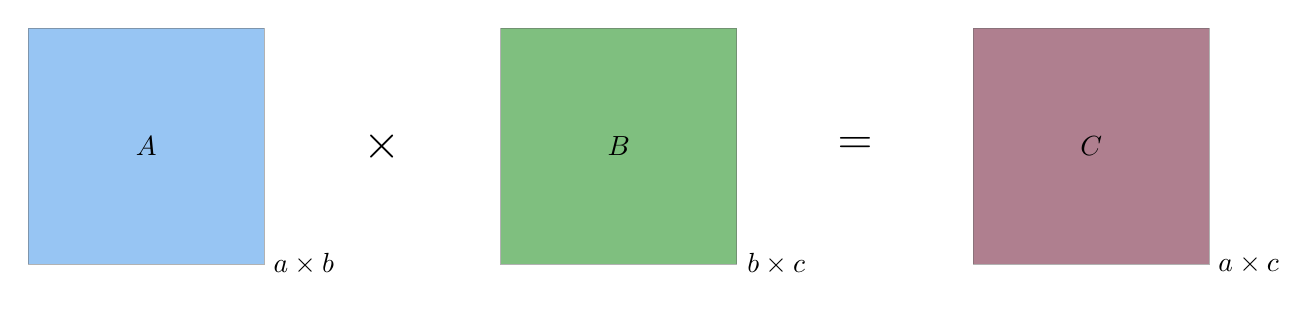
\begin{tikzpicture}
\definecolor{darkturquoise}{rgb}{0.0, 0.81, 0.82}


\node[rectangle,  draw = black!60, fill = bleudefrance, minimum height = 3 cm, minimum width = 3cm, opacity=.5, text opacity=1] (a) at (0,0) { $A$};

\node[] (dim_a) at (2,-1.5) { $a \times b$};

\node[] (times) at (3,0) {\LARGE $\times$};

\node[rectangle,  draw = black!60, fill = green!50!black, minimum height = 3cm, minimum width = 3cm, opacity=.5, text opacity=1] (b) at (6,0) { $B$};

\node[] (dim_b) at (8,-1.5) { $b \times c$};

\node[] (times) at (9,0) {\LARGE $=$};

\node[rectangle,  draw = black!60, fill = purple!50!black, minimum height = 3cm, minimum width = 3cm, opacity=.5, text opacity=1] (c) at (12,0) { $C$};

\node[] (dim_c) at (14,-1.5) { $a \times c$};




\end{tikzpicture}
}
% \end{figure}

\bigskip

\begin{itemize}
    \item<2-> Upload: $2ab + 2bc$ symbols of $\mathbb{F}_{4}$.
    
    \medskip
    
    \item<3-> Download: $4ac$ symbols of $\mathbb{F}_{4}$.
    
    \medskip
    
    \item<4-> Total Communication Rate: $ \mathcal{R} = \dfrac{ac}{2ab+2bc+4ac}$.

    \item<5-> Performs in $\mathbb{F}_4$ while DFT performs in $\mathbb{F}_5$.
\end{itemize}

\bigskip

\bigskip

\uncover<5->{
\textbf{$L=2$, $T=2$:} \textit{HerA} can performs still in $\mathbb{F}_4$ while DFT codes needs at least $\mathbb{F}_7$.
}
    
\end{frame}






\begin{frame}{Divide \& Parallelize (Inner Product Division)}

\begin{itemize}

\item Let $A \in \mathbb{F}_q^{a \times b}$ and $B \in \mathbb{F}_q^{b \times c}$.
    
\medskip
    
\item We divide $A$ and $B$ as  $A = \begin{bmatrix}
A_1 & \cdots & A_L
\end{bmatrix}$ and  $
B = \begin{bmatrix}
B_1 \\ \vdots \\ B_L
\end{bmatrix}.
$

\medskip

\item $AB = A_1 B_1 + \cdots + A_L B_L $

\medskip

\item<2-> Each server multiplies two matrices of dimensions $a\times \frac{b}{L}$ and $\frac{b}{L} \times c$.

\medskip

\item<3-> Correct choice of parameters allows for computational speedup.*

\end{itemize}

\uncover<3->{
\begin{textblock}{20}(0.1,14.7)
{\tiny \color{davysgrey} *R. G. L. D’Oliveira, S. El Rouayheb, D. Heinlein and D. Karpuk, \say{Notes on Communication and Computation in Secure Distributed Matrix Multiplication,} IEEE WPS, 2020.}
\end{textblock}
}

\end{frame}




\begin{frame}{Total Communication Rate for \textit{HerA} Scheme}

\begin{exampleblock}{Theorem}

\begin{itemize}
    \item Matrices being multiplied: $A \in \mathbb{F}_{q^2}^{a \times b}$ and $B \in \mathbb{F}_{q^2}^{b \times c}$
    \item<2-> Partitioning and security parameters: $L$ and $T$, such that $L+T \leq \frac{q^3}{2}$.
    \item<3-> Total amount of servers: $N = L + 2T$.
\end{itemize}

\uncover<4->{
Then, there exists a \textit{HerA} scheme which computes $AB$ with total communication rate

\begin{align*} 
\mathcal{R} = \left(\frac{Nb}{L} \left( \frac{1}{a}+\frac{1}{c} \right)+N\right)^{-1} .
\end{align*}
}
\end{exampleblock}   
\end{frame}



\begin{frame}{Conclusion and Open Problems}

\begin{itemize}
    \item  \textit{HerA} scheme achieves the same recovery threshold as in the literature while operating in smaller fields
    
    \medskip
    
    \item<2-> Given matrices in  $\mathbb{F}_{q^2}$ elements, are there schemes such that $L+T > \frac{q^3}{2}$?
    
    \medskip
    
    \item<3-> Lots of places for improvement.
    
    \medskip
    
    \item<3-> The general SDMM problem is still not well understood.
\end{itemize}
    
\end{frame}


\begin{frame}{}
  \centering \Large
  \emph{Thanks!}
\end{frame}



\end{document}
